\documentclass{beamer}

\usepackage{graphicx}
\usepackage{tikz}
\usepackage{multimedia}
\usepackage{fontspec}
\usepackage{ulem}
\usepackage{amsmath,amssymb,bm}

\RequirePackage{luatex85}


\setsansfont{texgyreheros}[
  Scale=MatchUppercase,% or MatchUppercase
  Extension=.otf,
  UprightFont=*-regular,
  ItalicFont=*-italic,
  BoldFont=*-bold,
  BoldItalicFont=*-bolditalic,
]

\defaultfontfeatures{Mapping=tex-text}

\setbeamerfont{frametitle}{family=\fontspec{Linux Biolinum}}

% Default theme as a base
\usetheme{default}

\definecolor{rr}{RGB}{56,200,0}
\definecolor{pp}{RGB}{101,42,138}
\definecolor{pr}{RGB}{0,161,255}
\definecolor{rp}{RGB}{255,39,39}

% Font
%\renewcommand\sfdefault{phv}
%\renewcommand\familydefault{\sfdefault}
%\setbeamerfont{title}{size=\Large}
%\setbeamerfont{frametitle}{size=\large}
%\setbeamercolor{frametitle}{bg=, fg=blue!70!black}
%\setbeamercolor{title}{bg=, fg=blue!70!black}
%\setbeamercolor{normal text}{bg=white, fg=black}

%\setbeamertemplate{footline}[frame number]

% Structure
\setbeamertemplate{itemize items}[default]
\setbeamertemplate{enumerate items}[circle]

%\setbeamertemplate{itemize item}[triangle]
\setbeamertemplate{itemize subitem}[circle]
\setbeamercolor{structure}{fg=black}
\setbeamercolor{item}{fg=RoyalBlue}
\setbeamercolor{itemize item}{fg=black}
\setbeamercolor{itemize subitem}{fg=black}
\setbeamercolor{itemize subsubitem}{fg=black}

\setbeamersize{text margin left=.5cm,text margin right=.5cm} 

% Features
\setbeamertemplate{headline}{}
\setbeamertemplate{navigation symbols}{}
%\setbeamertemplate{footline}{}

%\setbeamercolor{section in head/foot}{use=structure,bg=Blue!15!bg}
%\AtBeginDocument{%
%  {\usebeamercolor{section in head/foot}}
%  \pgfdeclareverticalshading{beamer@headfade}{\paperwidth}{%
%    color(0.0cm)=(bg); color(1.5cm)=(section in head/foot.bg) }
%  \setbeamercolor{section in head/foot}{bg=}
%}
%\addtoheadtemplate{\pgfuseshading{beamer@headfade}\vskip-1.5cm}{}

\newcommand{\mb}[1]{\mathbf{#1}}
\newcommand{\bs}[1]{\boldsymbol{#1}}
\newcommand{\gr}[1]{{\tiny\color{green!50!black} #1}}
\newcommand{\grb}[1]{{\small\color{green!50!black} #1}}
\newcommand{\cb}[1]{{\color{blue} #1}}
\newcommand{\crr}[1]{{\color{red} #1}}

\begin{document}



{
  \usebackgroundtemplate{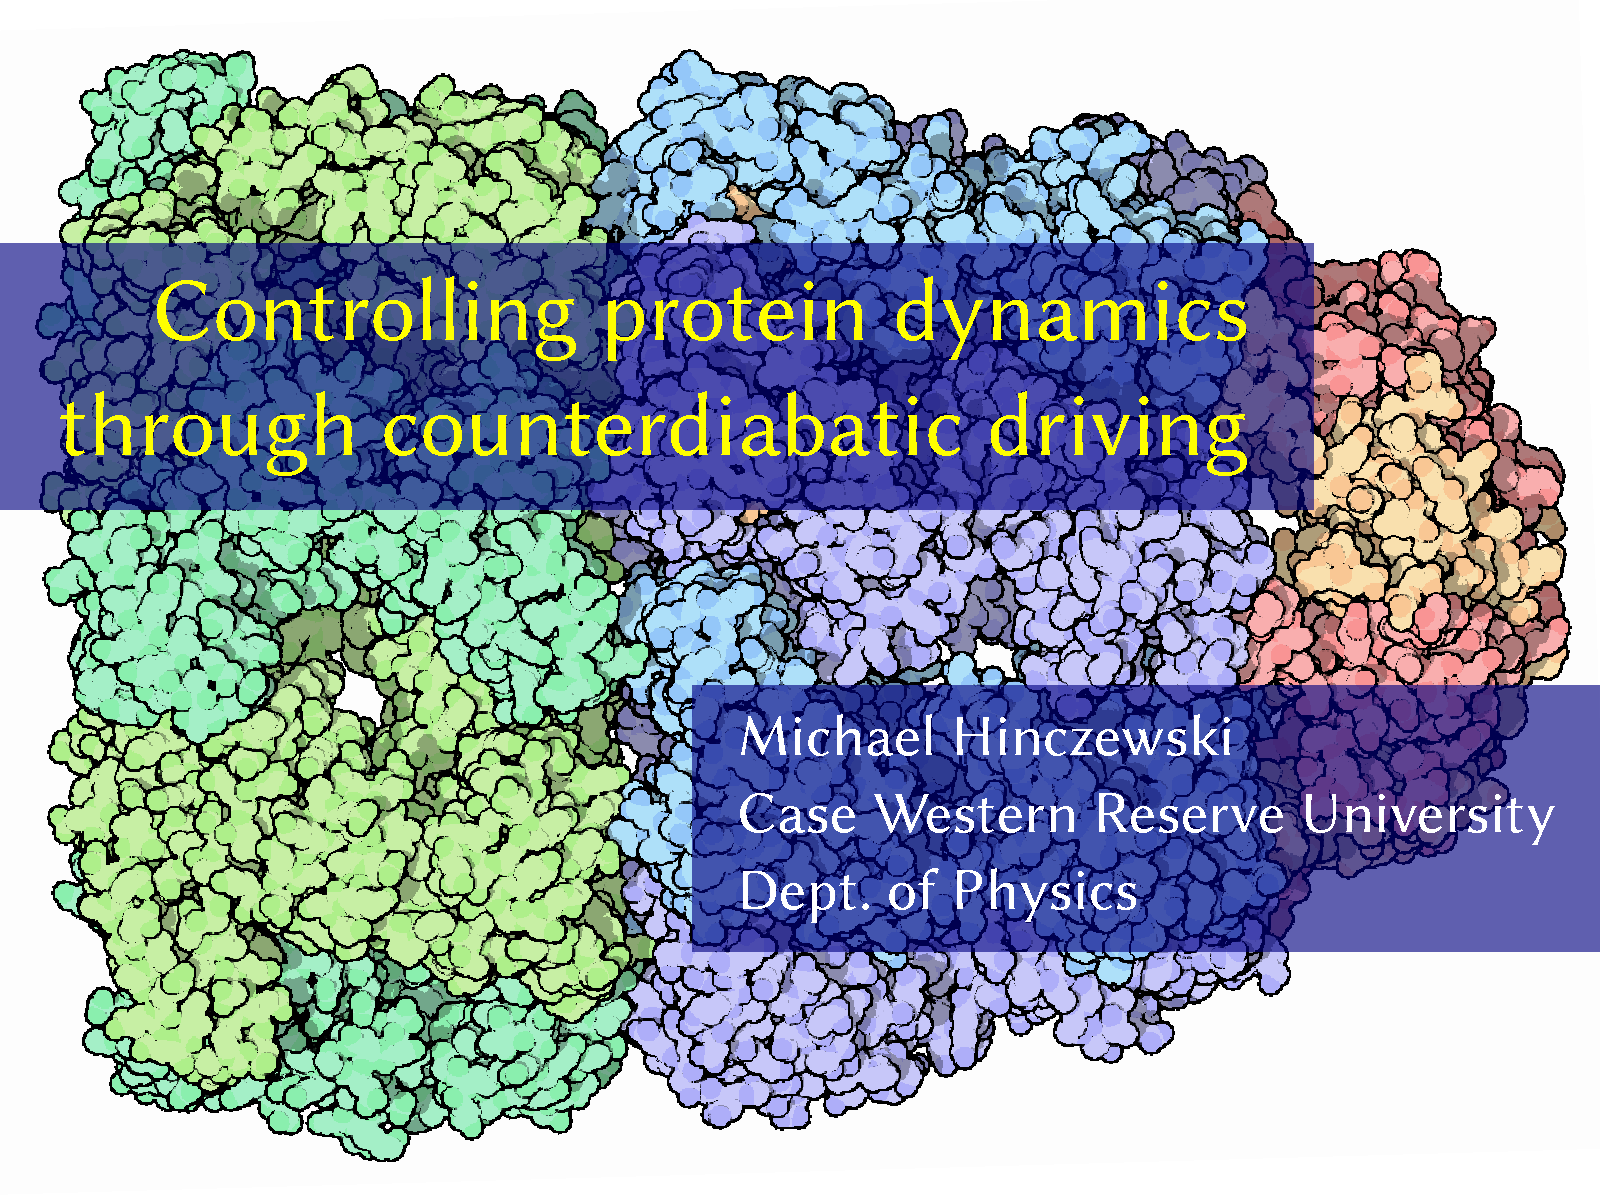
\includegraphics[width=\paperwidth]{title.pdf}}
\begin{frame}

\end{frame}
}


{
  \usebackgroundtemplate{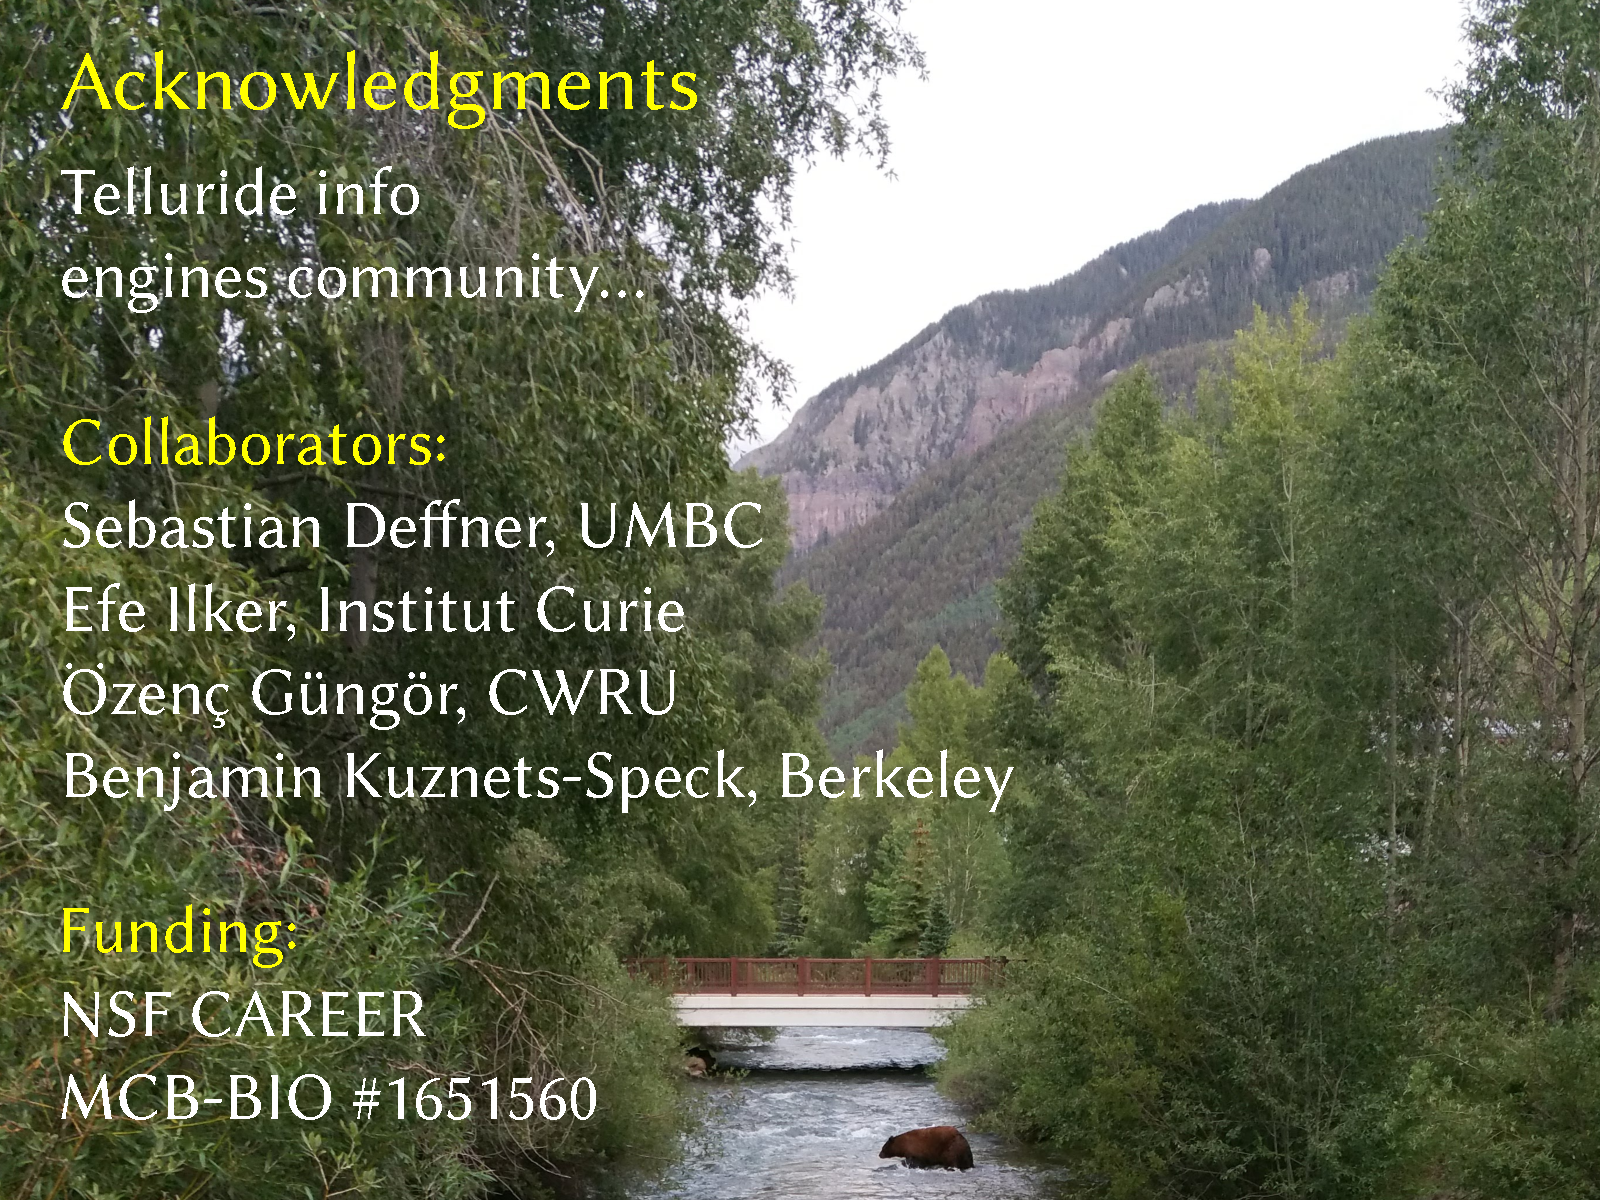
\includegraphics[width=\paperwidth]{acknow.pdf}}
\begin{frame}

\end{frame}
}

\begin{frame}{Shortcuts to adiabaticity}

  \begin{figure}
\includegraphics<1>[width=\textwidth]{analogy1.pdf}\includegraphics<2>[width=\textwidth]{analogy2.pdf}\includegraphics<3>[width=\textwidth]{analogy3.pdf}
  \end{figure}

\end{frame}


\begin{frame}{Traditional view of protein production}

  \begin{figure}
    \includegraphics<1>[width=\textwidth]{dogma1.pdf}\includegraphics<2>[width=\textwidth]{dogma1b.pdf}\includegraphics<3>[width=\textwidth]{dogma2.pdf}
  \end{figure}
  
\end{frame}

\begin{frame}{Proteins function at the cliff edge of unfolding}

  \begin{columns}
    \column{0.5\textwidth}
  \begin{figure}
    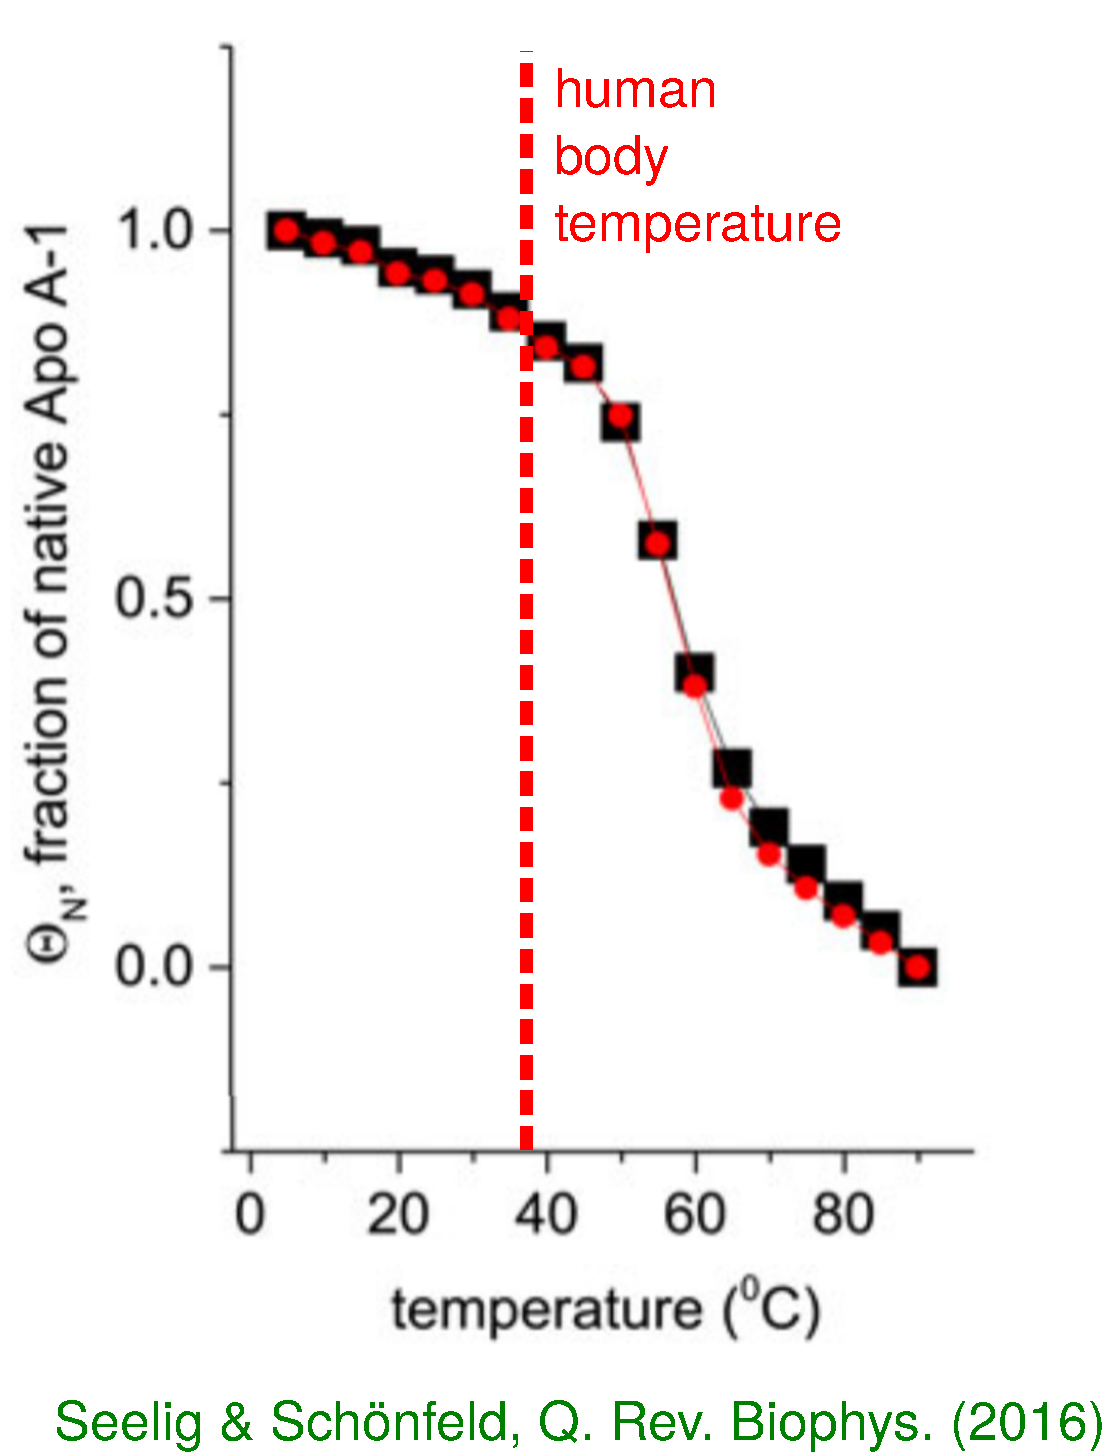
\includegraphics[width=\textwidth]{thermal_unfold.pdf}
  \end{figure}

  \pause
  \column{0.45\textwidth} Being on the verge of melting gives proteins
  the {\color{blue}dynamical flexibility} essential for their diverse roles as enzymes.

  \pause

  \vspace{1em}
  
  But it also makes them highly vulnerable to changes in temperature
  (even of a few degrees):  {\color{red} heat shock}.
  \end{columns}
\end{frame}

\begin{frame}{Constant threats: misfolding and aggregation}

  \begin{figure}
    \includegraphics<1>[width=\textwidth]{misfolding1.pdf}\includegraphics<2>[width=\textwidth]{misfolding2.pdf}\includegraphics<3>[width=\textwidth]{misfolding3.pdf}
  \end{figure}
\end{frame}

\begin{frame}{The protein ``hospital'':  possible chaperone pathways}
  \vspace{0.5em}
  \begin{figure}
\centering    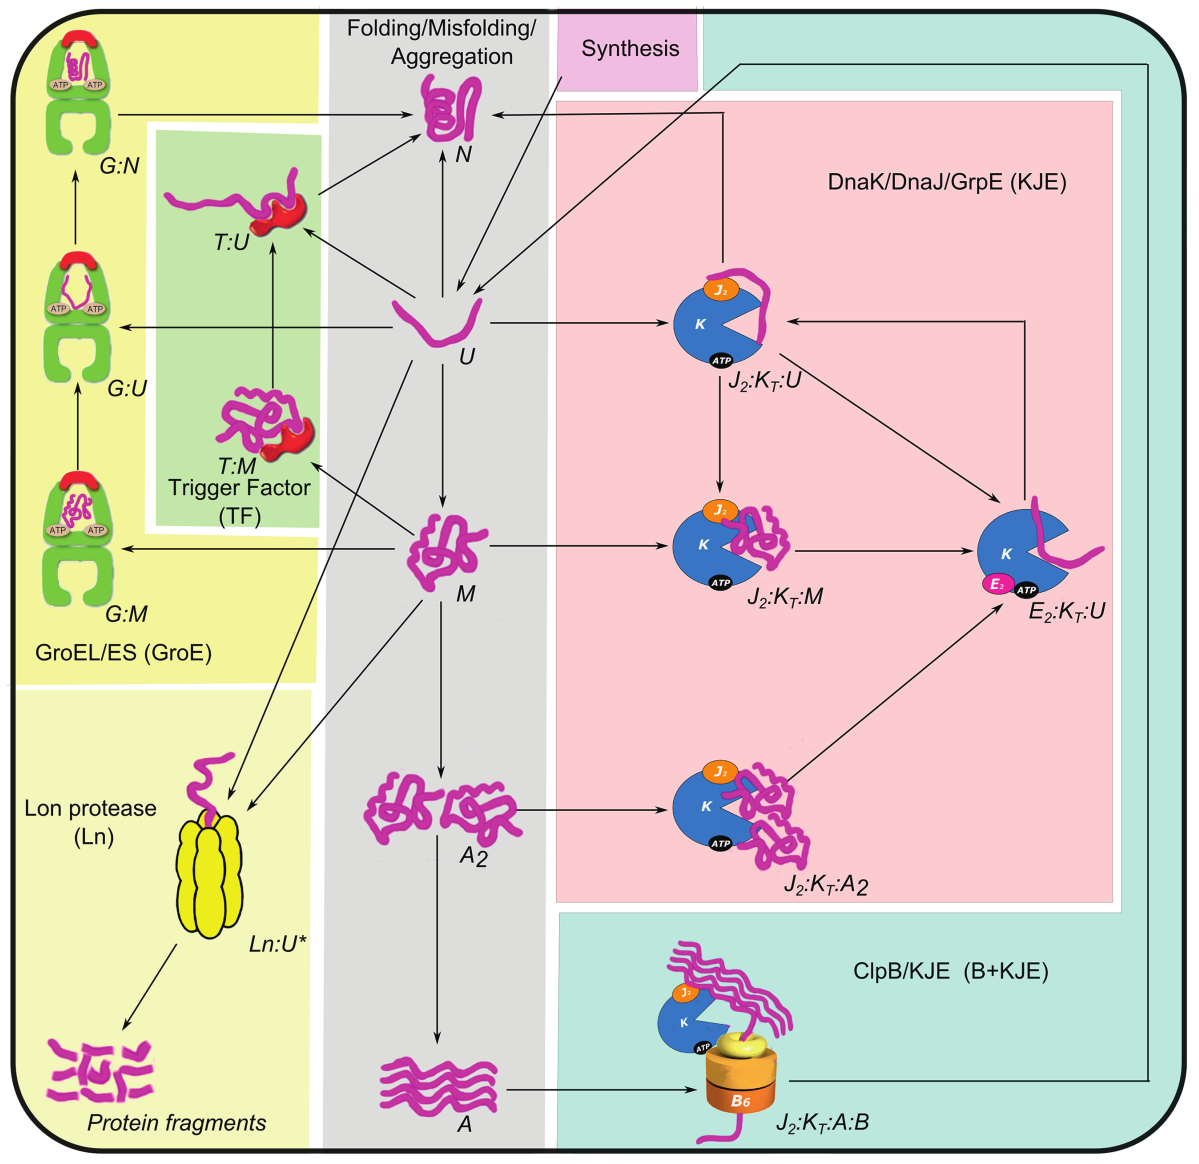
\includegraphics[width=0.65\textwidth]{ecoli_network.png}\\
      {{\it E. coli} chaperone network: \color{green!50!black}Santra {\it et al.}, PNAS (2017)}
  \end{figure}
\end{frame}

\begin{frame}{The protein ``hospital'':  possible chaperone pathways}

  \vspace{0.5em} Different classes of proteins interact primarily with
  different chaperone sub-systems:
  \begin{figure}
    \centering
    \includegraphics<1>[width=\textwidth]{ecoli_flux1.png}\includegraphics<2>[width=\textwidth]{ecoli_flux2.png}\includegraphics<3>[width=\textwidth]{ecoli_flux3.png}\\[1em]
 {\color{green!50!black}Santra {\it et al.}, PNAS (2017)}
  \end{figure}

  \pause\pause
      {\color{red} Under optimal growth conditions, chaperones are nearly fully occupied by ``patient'' proteins:  spare capacity is too energetically costly.}
  
\end{frame}


\begin{frame}{Heat shock}

  {What happens when the cell enters a higher temperature environment?\\[1em]}

  \pause

{\small  Functional classes of upregulated genes in yeast after a heat shock from 25$^\circ$C to 35$^\circ$C over 10 min (out of total of 91 genes upregulated by more than 2.8x):}
  \vspace{1em}
  \begin{figure}
    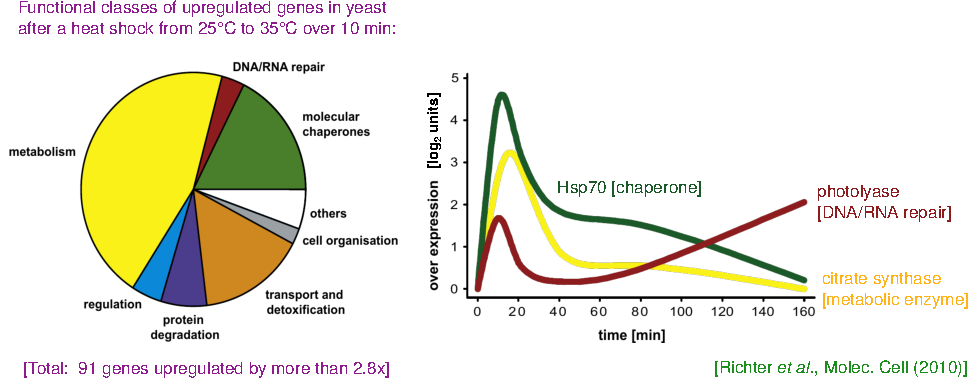
\includegraphics[width=\textwidth]{yeast_response.pdf}
  \end{figure}

  \pause

\alert{\small Can we understand this upregulation of chaperones using ideas from thermodynamic control?}

\end{frame}

\begin{frame}{Markov model for chaperone-protein interaction}

  \vspace{-1em}
  \begin{columns}
    \column{0.55\textwidth}
    \includegraphics<1>[width=\textwidth]{markov0.pdf}\includegraphics<2>[width=\textwidth]{markov0b.pdf}
    \column{0.42\textwidth} Using separation of timescales we can
    construct a simplified {\color{blue} Markov model} for a protein that tends to
    misfold under heat shock, focusing on four key states.
    \end{columns}
\end{frame}

\begin{frame}{Markov model for chaperone-protein interaction}

  \vspace{-1em}
  \begin{columns}[T]
    \column{0.5\textwidth}
    \centering
    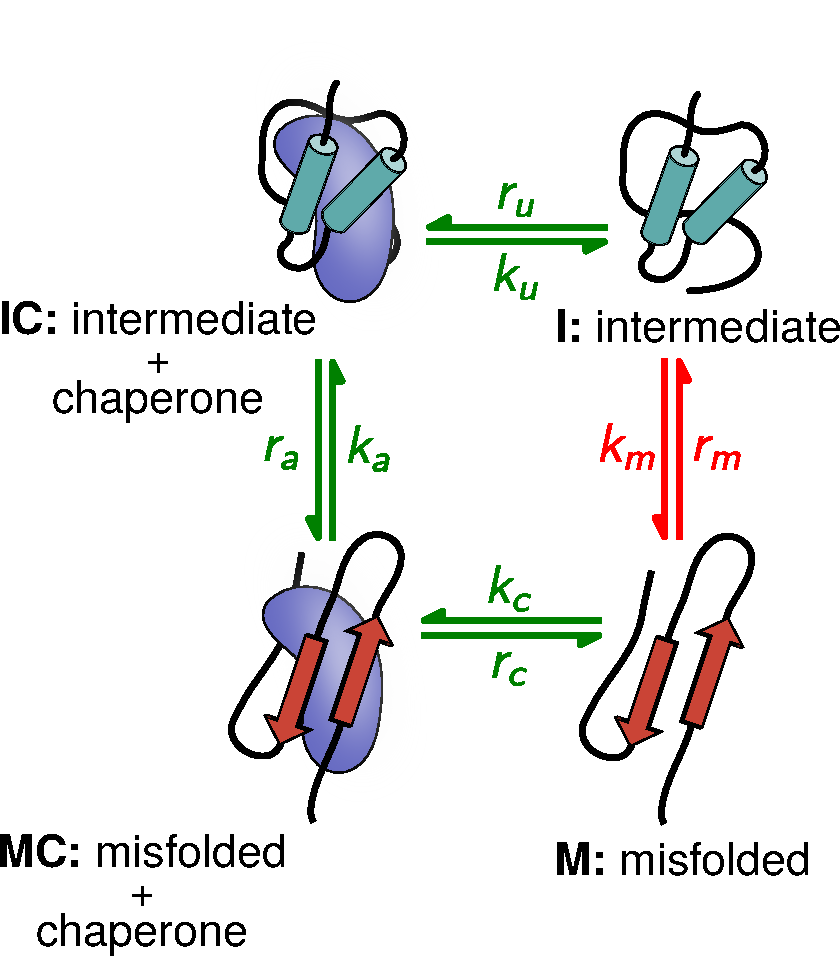
\includegraphics[width=0.95\textwidth]{markov1.pdf}\\[0.5em]
    {\small{\color{blue} \underline{Typical parameter values:}\\ $k_m = 10$ s$^{-1}$, $\epsilon = 10$ $k_B T$}}
    \column{0.47\textwidth} \vspace{0.5in} {\small We assume the system is undergoing heat
    shock, where conditions favor the misfolded over the intermediate
    state:
    \[
    \frac{k_m}{r_m} = e^{\beta \epsilon} \gg 1
    \]
    where $\epsilon >0$ is the free energy difference between the I
    and M states.\\[1em]}

    
    \end{columns}
\end{frame}

\begin{frame}{Markov model for chaperone-protein interaction}

  \begin{columns}[T]
    \column{0.5\textwidth}
    \centering
    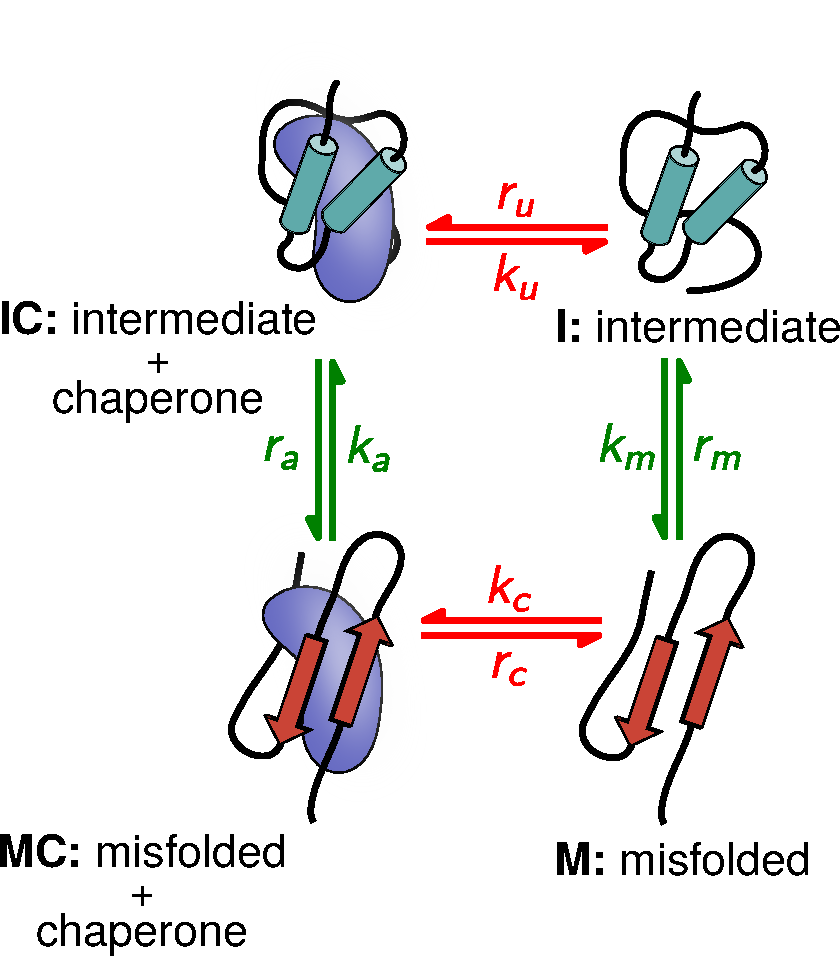
\includegraphics[width=0.95\textwidth]{markov2.pdf}\\[0.5em]
        {\small{\color{blue} \underline{Typical parameter values:}\\ $\gamma_c = 10^6$ M$^{-1}$s$^{-1}$, $\gamma_u =  10^4$ M$^{-1}$s$^{-1}$, $r_c = 5 \times 10^{-3}$ s$^{-1}$, $k_u = 0.2$ s$^{-1}$}}

    \column{0.47\textwidth} \vspace{0.5in} {\small Binding rates depend on free chaperone
    concentration $C$:
    \[
    k_c = \gamma_c C, \qquad r_u = \gamma_u C
    \]
    where usually $\gamma_c \gg \gamma_u$ (chaperone favors binding
    to misfolded states).\\[1em]}
    \end{columns}
\end{frame}

\begin{frame}{Markov model for chaperone-protein interaction}

  \vspace{0.5em}
  \begin{columns}
    \column{0.5\textwidth}
    \centering
    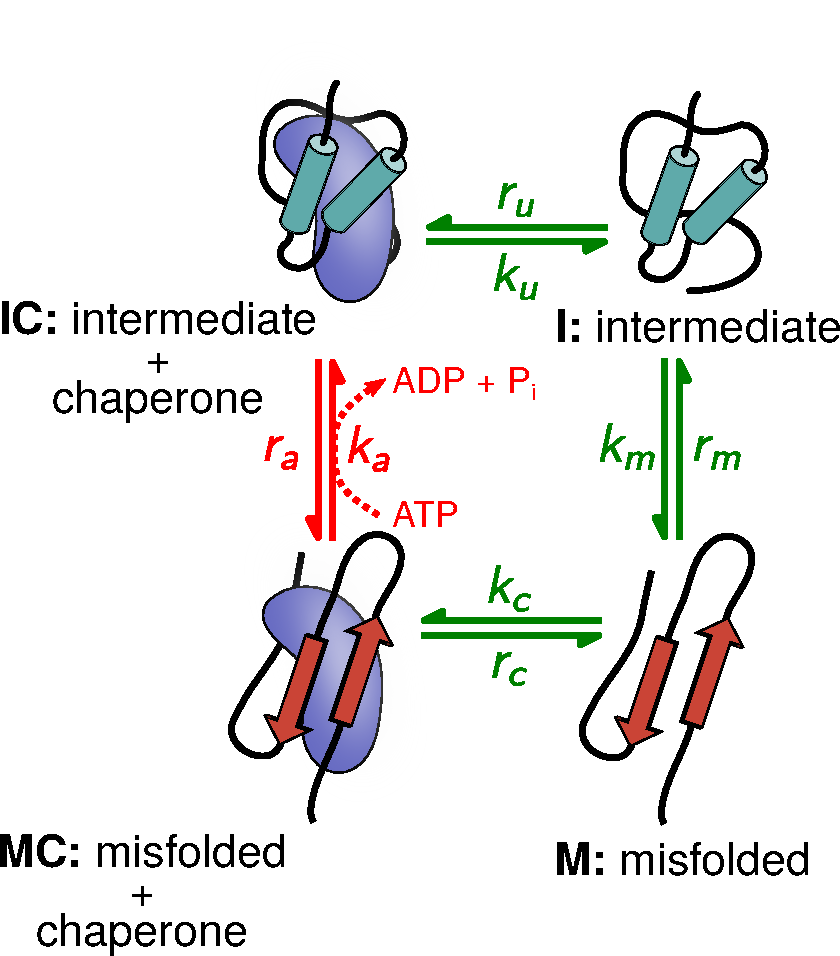
\includegraphics[width=0.95\textwidth]{markov3.pdf}\\[0.5em]
    {\small{\color{blue} \underline{Typical parameter values:}\\
$k_\text{f,cat} = 10^{-2}$ s$^{-1}$, $K_\text{f,M} = 400$ $\mu$M,\\ $A = 1$ mM, $B=0.1$ mM, $\Delta \mu = 22$ $k_BT$}}

    \column{0.47\textwidth} {\small Chaperone-catalyzed reactions
      follow Michaelis-Menten kinetics that depend on \alert{ATP concentration $A$} and
      \alert{ADP concentration $B$}:
    \[
k_a = \frac{k_\text{f,cat} A}{K_\text{f,M} + A}, \quad r_a = \frac{k_\text{r,cat} B}{K_\text{r,M} + B}
\] \\

\pause
{\color{green!50!black} Local detailed balance} leads to two constraints: the ``Haldane relation'',
\[
\frac{k_\text{f,cat} K_\text{r,M} \gamma_c k_u}{k_\text{r,cat} K_\text{f,M} \gamma_u r_c} = e^{-\beta \epsilon}
\]
and
\[
\frac{k_m \gamma_c k_a k_u}{r_m r_c r_a \gamma_u} = e^{\beta \Delta \mu}
\]
where $\Delta \mu= \Delta \mu_0 + k_BT {\sf ln} (A/B)$ is the ATP hydrolysis chemical potential.}

    \end{columns}
\end{frame}

\begin{frame}{Markov model: dynamics}

  \vspace{0.5em}
  \begin{columns}[T]
    \column{0.42\textwidth}
    \centering
    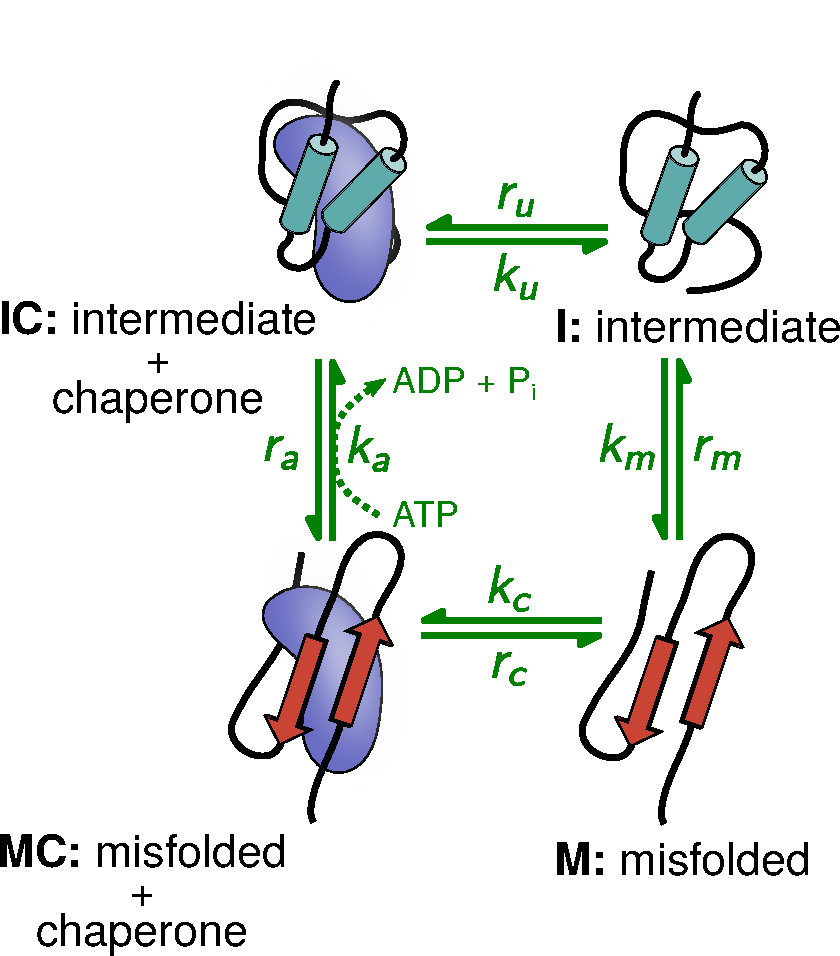
\includegraphics[width=\textwidth]{markov4.pdf}
    \column{0.55\textwidth}
    The state probabilities
    \[
    \bm{p}(t) = (p_M(t),p_{MC}(t),p_{IC}(t),p_I(t))
    \]
    obey the master equation
    \[
    \dot{\bm{p}}(t) = \Omega \bm{p}(t)
    \]
    with transition matrix
    \[
    \begin{split}
&\Omega =\\
&\left(\begin{smallmatrix} 
-k_c(C) -r_m & r_c & 0 & k_m \\ 
k_c(C) & -r_c -k_a(A) & r_a(B) & 0\\
0 & k_a(A) & -r_a(B) - k_u & r_u(C)\\
r_m & 0 & k_u & -k_m - r_u(C)
      \end{smallmatrix}\right)
      \end{split}
    \]
    \pause

For given $A$, $B$, $C$, the {\color{blue} stationary distribution} $\bm{\rho}$ satisfies: $\Omega \bm{\rho} = 0$.

    \end{columns}
\end{frame}

\begin{frame}{Chaperone upregulation as a control problem}

  \begin{columns}[T]
    \column{0.6\textwidth}
    \includegraphics<1-3>[width=\textwidth]{protocol1.pdf}\includegraphics<4>[width=\textwidth]{protocol1b.pdf}\includegraphics<5>[width=\textwidth]{protocol2.pdf}\includegraphics<6-7>[width=\textwidth]{protocol3.pdf}
    \column{0.39\textwidth} \only<1-3>{\vspace{1em}Right after heat shock, system
      relaxes quickly to stationary state for free chaperone
      concentration $C_0$.\\[1em]

      \pause
      There are insufficient chaperones available, so probability of being misfolded is high.\\[1em]

      \pause
      We would like to {\color{blue} drive the system to a new stationary state} with less misfolidng by increasing chaperone concentration to some $C_\tau$.}

    \only<7>{\vspace{1em}For a given $\rho_M(C_t)$, can we effectively eliminate the lag, so that $p_M(t) = \rho_M(C_t)$ at all $t$?\\[1em]
      
    \alert{Answer: Yes, via a counterdiabatic protcol.}}
  \end{columns}
    
\end{frame}

\begin{frame}{Counterdiabatic protocols for Markov models}

  \vspace{0.5em}
  {\color{blue} Ingredients:}
  \begin{itemize}
  \item  $N$ state Markov model with transition matrix $\Omega(\lambda_t)$ that depends on time-dependent control parameter(s) $\lambda_t$ for $0 \le t \le \tau$
    \vspace{0.25em}

    \pause
    
  \item Master equation for state probabilities $\bm{p}(t)$:
    \[
    \dot{\bm{p}}(t) = \Omega(\lambda_t) \bm{p}(t)
    \]

    \pause

  \item Instantaneous stationary state $\bm{\rho}(\lambda_t)$ defined via:
    \[
\Omega(\lambda_t) \bm{\rho}(\lambda_t) = 0
\]

  \end{itemize}

  \pause 
  {\color{red} Problem:} Find counterdiabatic transition matrix $\tilde{\Omega}(\lambda_t,\dot\lambda_t)$ such that $\bm{\rho}(\lambda_t)$ is a solution to the new master equation:
    \[
\dot{\bm{\rho}}(\lambda_t) = \tilde{\Omega}(\lambda_t,\dot\lambda_t) \bm{\rho}(\lambda_t)
    \]
  
\end{frame}

\begin{frame}{Solving the CD problem}
  
  {\color{red} Solution:} Infinitely many CD solutions for $\tilde{\Omega}(\lambda_t,\dot\lambda_t)$.  But most of them may be physically unrealizable in a given system.

  \pause
  \vspace{1em} In our case, the external control parameter is
  $\lambda_t = C_t$, and we work in the limit of large $k_m$, small
  $r_a$, so $\Omega(C_t)$ is approximately:
    \[
    \begin{split}
&\Omega(C_t) \approx \left(\begin{smallmatrix} 
{\color{blue} -k_c(C_t)} -r_m & r_c & 0 & k_m \\ 
{\color{blue} k_c(C_t)} & -r_c -{\color{blue} k_a(A)} & 0 & 0\\
0 & {\color{blue} k_a(A)} & - k_u & {\color{blue} r_u(C_t)}\\
r_m & 0 & k_u & -k_m - {\color{blue} r_u(C_t)}
      \end{smallmatrix}\right)
      \end{split}
    \]
    Really only {\color{blue} two knobs for control:}
    \begin{itemize}
      \item free chaperone concentration $C_t$\\
      \item ATP concentration $A$ (fixed in original protocol)
     \end{itemize}

\end{frame}

\begin{frame}{Solving the CD problem}

  Approximate CD solution $\tilde{\Omega}(C_t,\dot{C}_t)$ takes the form:
    \[
    \begin{split}
&\tilde{\Omega}(C_t,\dot{C}_t) \approx \left(\begin{smallmatrix} 
{\color{blue} -k_c(\tilde{C}_t)} -r_m & r_c & 0 & k_m \\ 
{\color{blue} k_c(\tilde{C}_t)} & -r_c -{\color{blue} k_a(\tilde{A}_t)} & 0 & 0\\
0 & {\color{blue} k_a(\tilde{A}_t)} & - k_u & {\color{blue} r_u(\tilde{C}_t)}\\
r_m & 0 & k_u & -k_m - {\color{blue} r_u(\tilde{C}_t)}
      \end{smallmatrix}\right)
      \end{split}
    \]
    where
    \[
    \begin{split}
    \tilde{C}_t &\approx C_t -\underbrace{\frac{\dot{C}_t}{\gamma_c}\frac{d}{d C_t}\ln \rho_M(C_t)}_{\text{\color{red} CD correction term}}\\
    k_a(\tilde{A}_t) = \frac{k_\text{f,cat} \tilde{A}_t}{K_\text{f,M}+\tilde{A}_t} &\approx k_a(A) - \underbrace{\frac{k_a(A) \rho_M(t) \dot{C}_t}{k_u(1-\rho_M(t))}\frac{d}{dC_t}\ln \rho_M(C_t)}_{\text{\color{red} CD correction term}}
    \end{split}
    \]

      
\end{frame}

\begin{frame}{CD protocol}
  \begin{figure}
\includegraphics<1>[width=\textwidth]{protocol_cd1.pdf}\includegraphics<2>[width=\textwidth]{protocol_cd2.pdf}
  \end{figure}
\end{frame}

\begin{frame}{CD protocols for different $\tau$}
  \begin{figure}
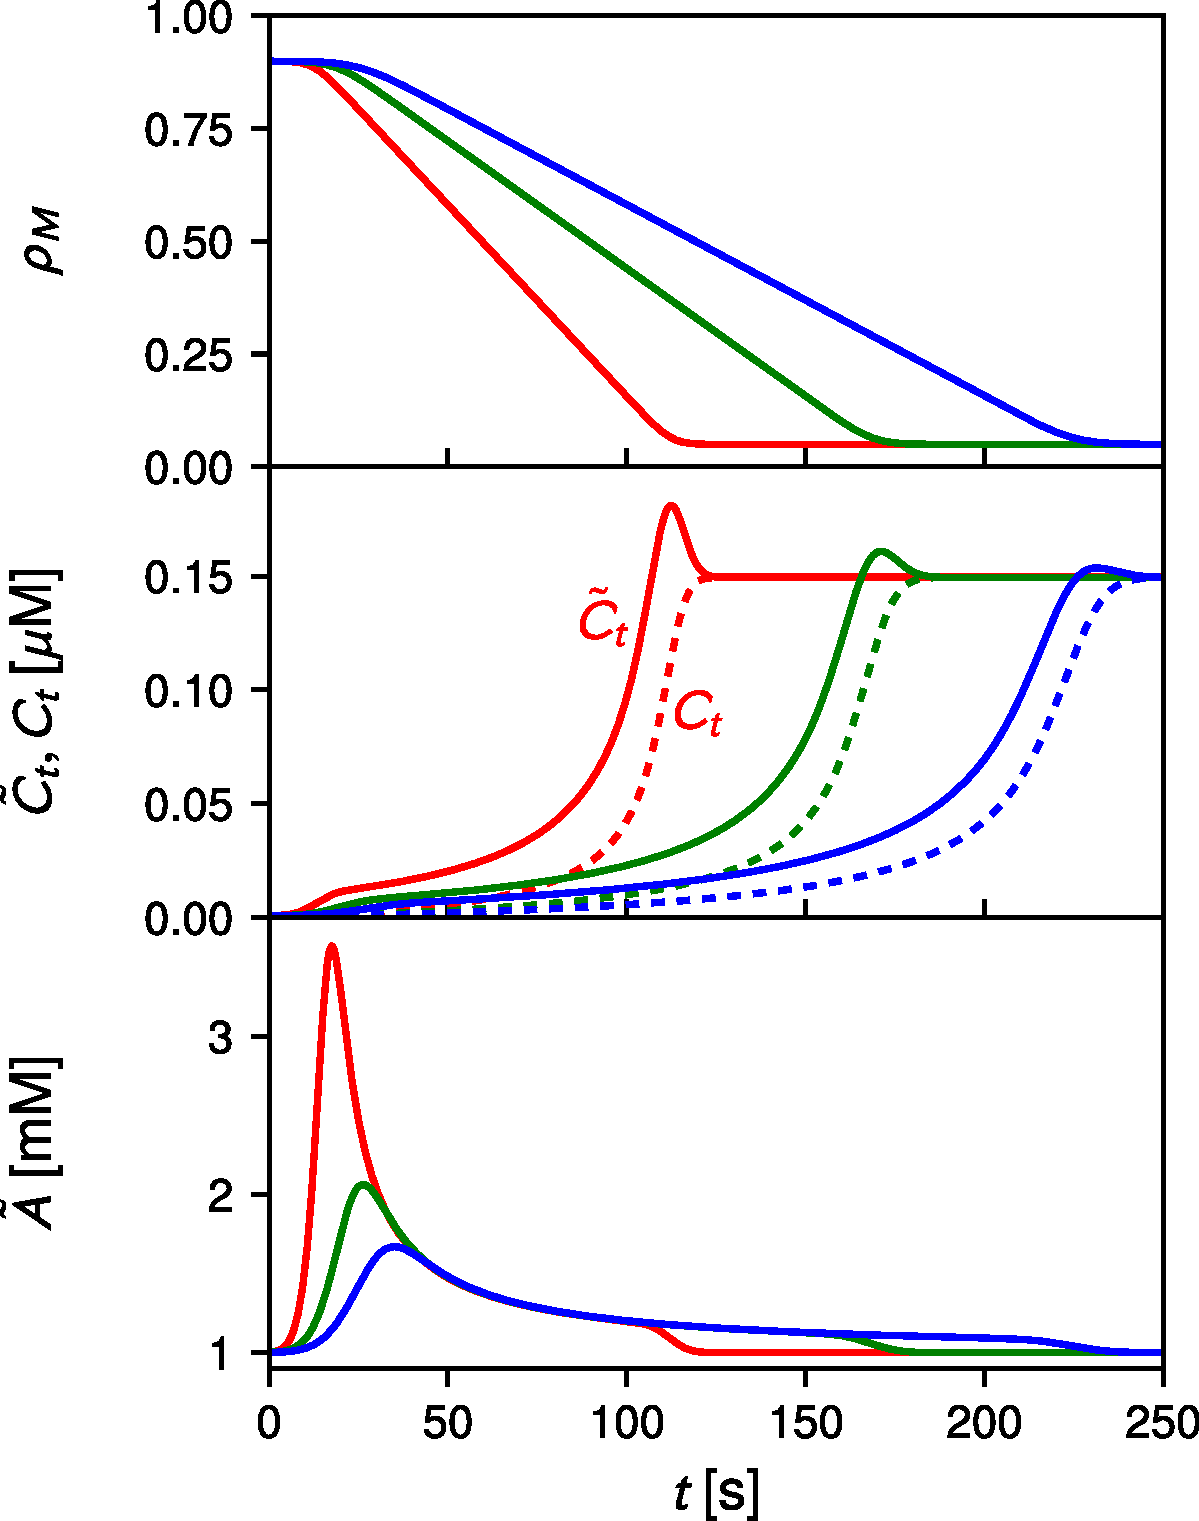
\includegraphics[width=0.53\textwidth]{cd_compare.pdf}
  \end{figure}
\end{frame}



\begin{frame}{Experimental data: {\it E. coli} heat shock response}

  \vspace{0.25em}
  \begin{figure}
    \centering
    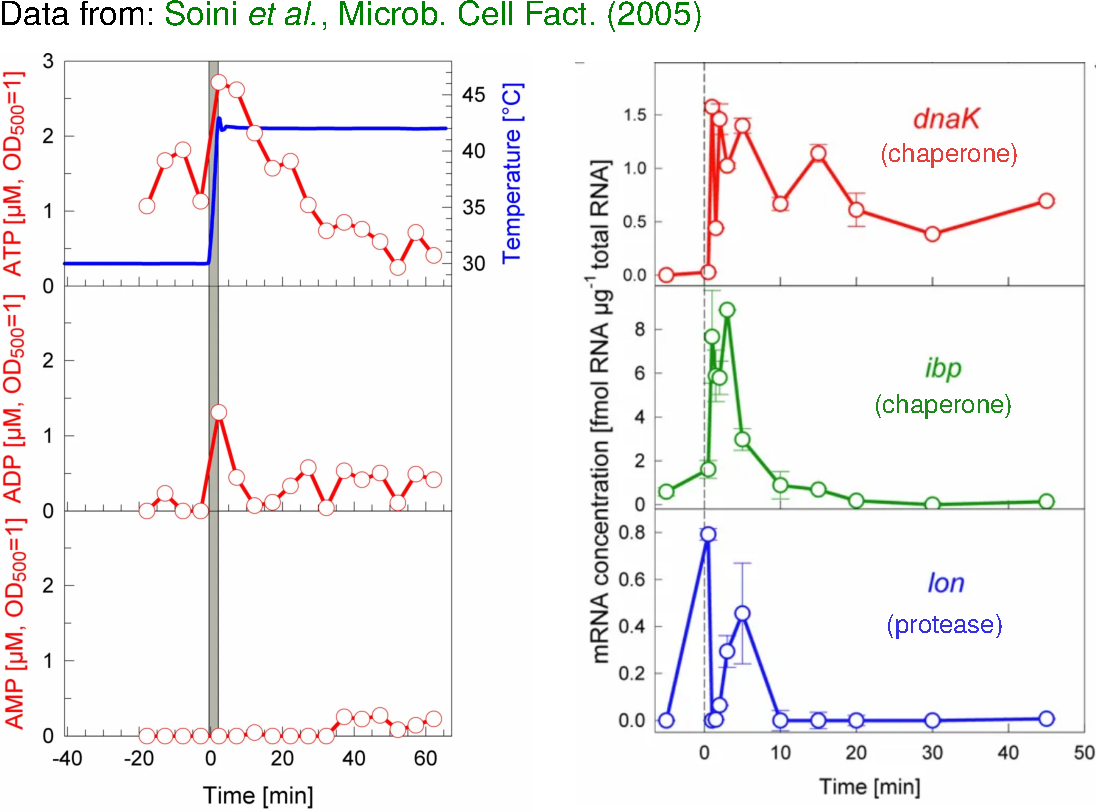
\includegraphics[width=0.95\textwidth]{exper.pdf}
    \end{figure}
\end{frame}

\begin{frame}{Extension:  from discrete states to the continuum}

  \begin{figure}
    \centering
    
\includegraphics[width=0.6\textwidth]{oned.pdf}
  \end{figure}

  \begin{center}
  Markov dynamics on chain of states\\
  $\Rightarrow$ continuum  Fokker-Planck description
\end{center}

  \pause
  \begin{itemize}

  \item We can recover Fokker-Planck counterdiabatic solution of {\color{green!50!black} Patra \& Jarzynski, New J. Phys. (2017)}.\\[1em]

    \pause
    
    \item Generalize solution to problems with position-dependent
      diffusivity (i.e. population genetics, force spectroscopy)

   \end{itemize}
\end{frame}

\begin{frame}{AFM force spectroscopy to study biomolecular complexes}

  \vspace{1em}
  \begin{figure}
    \centering
    \includegraphics<1>[width=0.95\textwidth]{afm_setup1.pdf}\includegraphics<2>[width=0.95\textwidth]{afm_setup2.pdf}\includegraphics<3>[width=0.95\textwidth]{afm_setup3.pdf}\includegraphics<4>[width=0.95\textwidth]{afm_setup4.pdf}
  \end{figure}

\end{frame}

\begin{frame}{Counterdiabatic driving to correct nonadiabatic artifacts}

  \begin{columns}[T]
    \column{0.38\textwidth}
    \includegraphics<1>[width=\textwidth]{pulling_results0.pdf}\includegraphics<2>[width=\textwidth]{pulling_results.pdf}
    \column{0.6\textwidth}

    \vspace{1em}
    
    Fast pulling leads to rupture distributions
    far from those predicted by adiabatic theories.\\[1em]

    Parameter extraction for bond lifetime vs. force:
    \[
    \tau(F) = \tau_0 \,\text{exp}(-d F)
    \]

    \vspace{1em}
    
    \begin{tabular}{l|ll}
      & $\tau_0$ [s] & $d$ [nm]\\\hline
      {\color{red} measured:} & 0.84 & 0.52\\
      {\color{magenta!50!black} expected:} & 10 & 0.40\\
      \pause
      {\color{blue} with CD:} & 9.74 & 0.40\\
    \end{tabular}

    \vspace{1em}
      {\color{blue}  CD protocol just depends on measurable properties of the AFM cantilever and handles, independent of the complex.}

  \end{columns}
\end{frame}

\begin{frame}{Future work}

  Testing these ideas out experimentally:\\[1em]

  \begin{itemize}

    \item Generalizing to more realistic models, and checking for
      biological realizations of CD protocols in heat shock
      experimental data.\\[1em]

      \pause
      
    \item Analogous methods should work for any enzymatic reaction
      cycle: a ``straightforward'' proof-of-principle experiment?\\[1em]

      \pause

    \item Validating the AFM pulling CD protocol.

  \end{itemize}
\end{frame}

\begin{frame}{Counterdiabatic protocols for Markov models}

  \vspace{0.25em}
         {\color{red} Solution:} \[
         \tilde{\Omega}_{ij}(\lambda_t,\dot\lambda_t) = \hat{\Omega}_{ij}(\lambda_t,\dot\lambda_t) \Gamma_{j}(\lambda_t,\dot\lambda_t)\]
         where one constructs the matrix $\hat{\Omega}_{ij}$ and vector $\Gamma_i$ as follows:

         \begin{overlayarea}{\textwidth}{4in}
         
\only<2>{{\bf\color{blue}{ Step 1:}} Construct $\hat{\Omega}_{ij}$,
\[
\hat{\Omega}_{ij}(\lambda_t,\dot\lambda_t) = \tilde{M}_{ij}(\lambda_t,\dot\lambda_t)/\rho_j(\lambda_t)\]
where $\tilde{M}$ is an arbitrary matrix with positive off-diagonal elements where each row and each column sum to zero.  {\color{blue}Each choice of $\tilde{M}$ corresponds to a distinct CD protocol.}}

\only<3-4>{{\bf\color{blue}{ Step 2:}} Construct $\Gamma_i(\lambda_t,\dot\lambda_t)$,
  \vspace{-0.5em}
    \[
    \Gamma_i(\lambda_t,\dot\lambda_t) = \frac{\left(\hat{\Omega}^\times(\lambda_t,\dot\lambda_t) \dot{\bm{\rho}}(\lambda_t)\right)_i}{\rho_i(\lambda_t)} + \Gamma_0(\lambda_t,\dot\lambda_t)
    \]
    \vspace{-0.5em}

    \begin{overlayarea}{\textwidth}{2in}
    \only<4>{
    Here $\hat{\Omega}^\times$ is the Drazin pseudoinverse of $\hat{\Omega}$, which satisfies:
    \[
    \hat{\Omega}^\times(\lambda_t,\dot\lambda_t) \hat{\Omega}(\lambda_t,\dot\lambda_t) = I - \bm{\rho}(\lambda_t) \bm{e}^T
    \]
    
    \vspace{-0.5em}
    where $I$ is the identity matrix and $e_i = 1$ for all $i$.  $\Gamma_0$ is uniquely specified by enforcing the condition:\\[-0.5em]
    \[
    \sum_{i=1}^N \frac{\rho_i(\lambda_t)}{\Gamma_i(\lambda_t,\dot\lambda_t)}  = 1
    \]}
    \end{overlayarea}
}

\end{overlayarea}
\end{frame}

\begin{frame}{Constraints on possible CD protocols}

  Arbitrary $\tilde{M}$ \quad \Rightarrow \quad infinitely many CD protocols!

  \vspace{1em}
  \pause

  But for a specific system, almost none of them may be physically realizable.

  \pause

  \vspace{1em} {\color{red} Typical constraints:}

  \begin{itemize}
  \item {\color{blue} Continuity:} $\tilde{M}(\lambda_t,\dot\lambda_t)$ should be
    continuous in $t$.
    \vspace{0.25em}
    \pause

  \item {\color{blue} Boundary conditions:}  in order for $\tilde{\Omega}(\lambda_t,\dot\lambda_t) = \Omega(\lambda_t)$ at $t=0$ and $\tau$, we must have $\tilde{M}_{ij} = \Omega_{ij}\rho_j$ at those times.
    \vspace{0.25em}
    \pause


  \item {\color{blue} Controllability:} some elements of
    $\tilde{M}_{ij}$ may not be amenable to external control (i.e. the
    corresponding elements $\tilde{\Omega}$ cannot be varied).
  \end{itemize}

\end{frame}

\end{document}

